%
%
%
\begin{appendix}

%----------------------------------------------------------------------------
%----------------------------------------------------------------------------
%----------------------------------------------------------------------------
\newpage

\begin{center}
	\huge{Anhänge}
\end{center}

\normalsize

%----------------------------------------------------------------------------
%----------------------------------------------------------------------------
%----------------------------------------------------------------------------
\section{Modellumstellung}
{
Abschließend soll das das bisher verwendete Modell umgeschrieben werden, damit die Allgemeingültigkeit darin enthalten ist.
\begin{align}
%
%\mathbf{0}&=\mathbf{A}\mathbf{x}-\mathbf{b}\\
%
\mathbf{A}&=
\left(
	\begin{array}{cccccc}
		x_k-x_0 & y_k-y_0 & z_k-z_0 & \sum_{i=1,j=0}^{k}(-a_1\delta_{ij}) &  -a_2\Theta_0 & \sum_{i=1,j=0}^{k}(a_2\Theta_k\delta_{ij})
	\end{array}
\right)\nonumber\\
%
\mathbf{x}&=
\left(
   \begin{array}{c}
	   x-x_0\\
	   y-y_0\\
	   z-z_0\\
	   n_0^2-n_k^2\\
	   n_0\\
	   n_k
   \end{array}
\right)\nonumber\\
%
\mathbf{b}&=
	\begin{array}{c}
		a_{0k}-a_{3kj} 
	\end{array}
	= c_{kj}'\nonumber
\end{align}
%
Dabei steht $\delta_{ij}$ für den bekannten Kronecker-Operator und bedeutet:
\begin{equation*}
\delta_{ij} = \begin{cases}1 ~\text{für}~ i=j\\ 0 ~\text{für}~ i\neq j\end{cases}
\end{equation*}
%
Im Expliziten sehen die Matrix $\mathbf{A}$ und der Vektor $\mathbf{b}$, für denn Fall $N'=3$ und $k=\{1,2,3\}$, wie folgt aus:
%
\begin{multline}
\mathbf{A}=\\
\left(
	\begin{array}{cccccccccc}
		x_1-x_0 & y_1-y_0 & z_1-z_0 & -a_1 & 0 & 0 & -a_2\Theta_0 & a_2\Theta_3 & 0 & 0 \\
		x_2-x_0 & y_2-y_0 & z_2-z_0 & 0 & -a_1 & 0 & -a_2\Theta_0& 0 & a_2\Theta_3 & 0 \\
		x_3-x_0 & y_3-y_0 & z_3-z_0 & 0 & 0 & -a_1 & -a_2\Theta_0& 0 & 0 & a_2\Theta_3
	\end{array}
\right) \nonumber
\end{multline}
%
\begin{equation}
\mathbf{x}=
\left(
	\begin{array}{c}
		x-x_0	\\
		y-y_0	\\
		z-z_0	\\
		n_0^2-n_1^2	\\
		(\dots)	\\
		n_0^2-n_3^2	\\
		n_0 \\
		n_1	\\
		(\dots)	\\
		n_3	
	\end{array}
\right)\nonumber
\end{equation}
%
\subsubsection{Bemerkungen - Finales Modell}
%
Das Ergebnis ist eine $3\times10$ Matrix und ein $1\times10$ Vaktor. Es ist möglich diesem Modell eine beliebige Anzahl an Antennen hinzuzufügen. Fügt man eine Antenne zur Berechnung hinzufügen würde sich die Matrix $\mathbf{A}$ um zwei Spalten und eine Zeile erweitern, der Vektor $\mathbf{x}$ analog um 2 Zeilen.

}


\newpage
\section{test}
\begin{tikzpicture}[x=0.1,y=0.04cm]

  \def\xmin{3}
  \def\xmax{9.2}
  \def\ymin{2}
  \def\ymax{15.5}

  % grid
  \draw[style=help lines, ystep=2, xstep=1] (\xmin,\ymin) grid
  (\xmax,\ymax);

  % axes
  \draw[->] (\xmin,\ymin) -- (\xmax,\ymin) node[right] {$x$};
  \draw[->] (\xmin,\ymin) -- (\xmin,\ymax) node[above] {$y$};

  % xticks and yticks
  \foreach \x in {0,1,...,280}
    \node at (\x, \ymin) [below] {\x};
  \foreach \y in {0,1,...,2200}
    \node at (\xmin,\y) [left] {\y};

  % plot the data from the file data.dat
  % smooth the curve and mark the data point with a dot
  \draw[color=blue] plot[smooth,mark=*,mark size=1pt] file {data.dat}
   node [right] {data};

\end{tikzpicture}

%----------------------------------------------------------------------------
%----------------------------------------------------------------------------
%----------------------------------------------------------------------------
\newpage
\begin{landscape}
	\section{Projektlaufplan KW 23}
	\label{sec:projectplan}
	\scalebox{.75}{
		\input{common/documents/project_plan_KW22.tex}
		}
\end{landscape}

%----------------------------------------------------------------------------

\end{appendix}
